\section{Postulates of Quantum Physics - 量子物理的“公理”}
\subsection{Postulate 1 - “公理”一}
Quantum physics/mechanics are usually taught as a subsequent course of undergraduate classical physics course. In this course, however, we directly develop from the postulates to describe physics quantum-mechanically. \par
This includes describing the physics of particles (e.g. electrons, photons, single atoms), many-body systems, superconducting systems, which are small systems, and even large systems like the solar system or the entire universe. We may also wish to describe different degrees of freedom -- vectorial degrees of freedom (e.g. continuous degrees of freedom like \impt{position} or \impt{momentum}, and discrete/countable degrees of freedom like \impt{spin}), and scalar degrees of freedom (e.g. mass, charge, phase etc.). \par
To simplify our analyses, we may choose to describe certain degrees of freedom in a quantum mechanical way, and others classically. For example:
\begin{quote}
    Consider an electron, if we wish to understand its spin, we may model its spin quantum-mechanically while modelling its position or its related electromagnetic field classically. \\
    We consider this a \impt{hybrid model}.
\end{quote} \par
This motivates the first two postulates of quantum physics.
\begin{postulate}
    A \uimpt{quantum system} is associated with a \uimpt{complex Hilbert space $\hilbert$} (a.k.a the state space)
\end{postulate}
Mathematically, a Hilbert space is an inner product space over $\C$ that is complete:
\begin{quote}
    1. Completeness: every \impt{Cauchy sequence} converges. \\
    2. Inner product space over $\C$: the inner product is in a \impt{sesquilinear form} such that it is \impt{anti-linear} in the first argument. Specifically, if we define $(\cdot, \cdot)$ as the inner product, and $\lambda, \mu \in \C$, we have the properties:
    \begin{quote}
        2.1. $(\lambda \psi, \phi) = \lambda^{*} (\psi, \phi)$ \\
        2.2. $(\psi, \mu \phi) = \mu (\psi, \phi)$
    \end{quote}
\end{quote}
Then, we continue to the second postulate.
% ----------------------------------------------------------------
\subsection{Postulate 2 - “公理”二}
After associating a quantum system with a Hilbert space, we now wish to associate the states in such a quantum system with some mathematical object.
\begin{postulate}
    A \uimpt{quantum state} in a quantum system is mathematically represented by a \uimpt{normalized vector} $\psi$, such that $\psi \in \hilbert$.
\end{postulate}
This essentially gives us
$$\norm{\psi} = \sqrt{(\psi, \psi)} = 1$$
Furthermore, this also states that if a vector in such a Hilbert space is \textbf{not normalized}, it is \textbf{not a valid quantum state}. Only \textbf{normalized vectors} can be \textbf{quantum states}. Notice that right now, we have not used \impt{Dirac notation} to denote quantum states, we will do so later.
\subsubsection{Dirac Notation/Bra-ket Notation (Part 1) - 狄拉克记号(第一部分)}
To motivate the use of Dirac notations, we first consider an example of a \impt{qubit}, which is a two-level quantum system. This is saying, it is a quantum system with two dimensions (e.g. $\hilbert = \C^2$, with standard inner product definition). In such a system, an arbitrary quantum state can be
$$\psi = \begin{pmatrix} \alpha \\ \beta \end{pmatrix}, \abs{\alpha}^2 + \abs{\beta}^2 = 1$$
Then, an inner product between two states will be
$$(\psi, \psi^{'}) = \conj{\alpha}\alpha' + \conj{\beta}\beta'$$
In this quantum system, it is motivated to label the basis to be:
$$\ket{0} = \begin{pmatrix}
    1 \\ 0
\end{pmatrix}, \ket{1} = \begin{pmatrix}
    0 \\ 1
\end{pmatrix}$$
Meaning that
$$\psi = \begin{pmatrix}
    \alpha \\ \beta
\end{pmatrix} = \alpha \ket{0} + \beta \ket{1} \equiv \ketpsi$$
Furthermore, from this notation we have:
$$\ketpsi = \Sum{x = 0}{1} \psi(x)\ket{x}, \psi(0) = \alpha, \psi(1) = \beta$$
\begin{definition}
    Define the \uimpt{wavefunction} of a quantum state $\ketpsi$ to be:
    $$\psi: \{\text{basis labels}\} \to \C$$
    which is a function assigning coefficients of the vector to the basis vectors
\end{definition}
Notice that the vector $\ketpsi$ is not basis dependent, but its wavefunction (i.e. coefficient-assignment function) is basis dependent. \par
In the same system, we can also define two other basis states:
$$\ketplus = \frac{1}{\sqrt{2}}\begin{pmatrix}
    1 \\ 1
\end{pmatrix}, \ketminus = \frac{1}{\sqrt{2}}\begin{pmatrix}
    1 \\ -1
\end{pmatrix}$$
In this basis,
$$\psi = \alpha \ket{0} + \beta \ket{1} = \frac{\alpha + \beta}{\sqrt{2}}\ketplus + \frac{\alpha - \beta}{\sqrt{2}}\ketminus$$
This thus gives a different wavefunction:
\begin{align*}
    \tilde{\psi}: \{+, -\} &\to \C \\
    + &\mapsto \frac{\alpha + \beta}{\sqrt{2}} \\
    - &\mapsto \frac{\alpha - \beta}{\sqrt{2}}
\end{align*}
With the wavefunction defined for a quantum state, the inner product of these states is thus:
$$(\ketpsi, \ketphi) = \begin{cases}
    \displaystyle \Sumi{x} \conj{\psi}(x)\phi(x) & \dim \hilbert = n < \infty \\
    & \\
    \displaystyle \intR \conj{\psi}(x)\phi(x) \dx & \dim \hilbert = \infty
\end{cases}$$
Notice that as of right now, there are three uses of the symbol ``$\psi$'':
\begin{quote}
    1. $\psi \in \hilbert$: $\psi$ is a vector. \\
    2. $\ketpsi \in \hilbert$: $\psi$ is a name, or a label. \\
    3. $\psi: \{\text{basis labels}\} \to \C$: $\psi$ is a function, specifically the wavefunction for the state $\ketpsi$.
\end{quote}
\subsubsection{Dirac Notation/Bra-ket Notation (Part 2) - 狄拉克记号(第二部分)}
To further motivate the use of Dirac notations, apart from a finite-dimensional quantum system, we now consider a continous 1D system (i.e. think of 1D real space, $\R$), and we wish to model the position of a particle. In this case, we denote each position $x \in \R$ to be one physical state. This denotion is a bit ``iffy'', as each state is not strictly normalizable, but for now, we look over it. \par
For any analysis, we first define the quantum system, which in this case, define
$$\hilbert = \Span{\ketx}_{x \in \R}$$
In this case, we should have $\forall x \ne x' \in \R$, $\ketx, \ket{x'}$ should be distinguishable/orthogonal. This is to require:
$$(\ketx, \ket{x'}) = 0, (\ketx, \ketx) = 1$$
However, this requirement is only well-defined in a finite-dimensional space. Therefore, we instead ask for:
$$(\ketx, \ket{x'}) = \delta(x-x')$$
where $\delta$ is the \hyperref[subsec:dirac-delta]{\textcolor{cyan}{Dirac delta function}}. \par
In this quantum system, every quantum state $\ketpsi \in \hilbert$ can be written as a continuous linear combination of $\{\ketx\}_{x \in R}$
$$\ketpsi = \intR \psi(x)\ketx \dx$$
with normalization condition
$$\intR \conj{\psi}(x)\psi(x) \dx = 1$$
This indicates the wavefunction of quantum states in a system are \impt{square-integrable} and \impt{normalized}. An example of such a wavefunction is the \impt{Gaussian wavepacket}:
$$\psi(x) = e^{\imag k x} \cdot \frac{1}{\sqrt[4]{2\pi\sigma^2}} \cdot e^{-\frac{(x-x_0)^2}{4\sigma^2}}$$
\begin{center}
    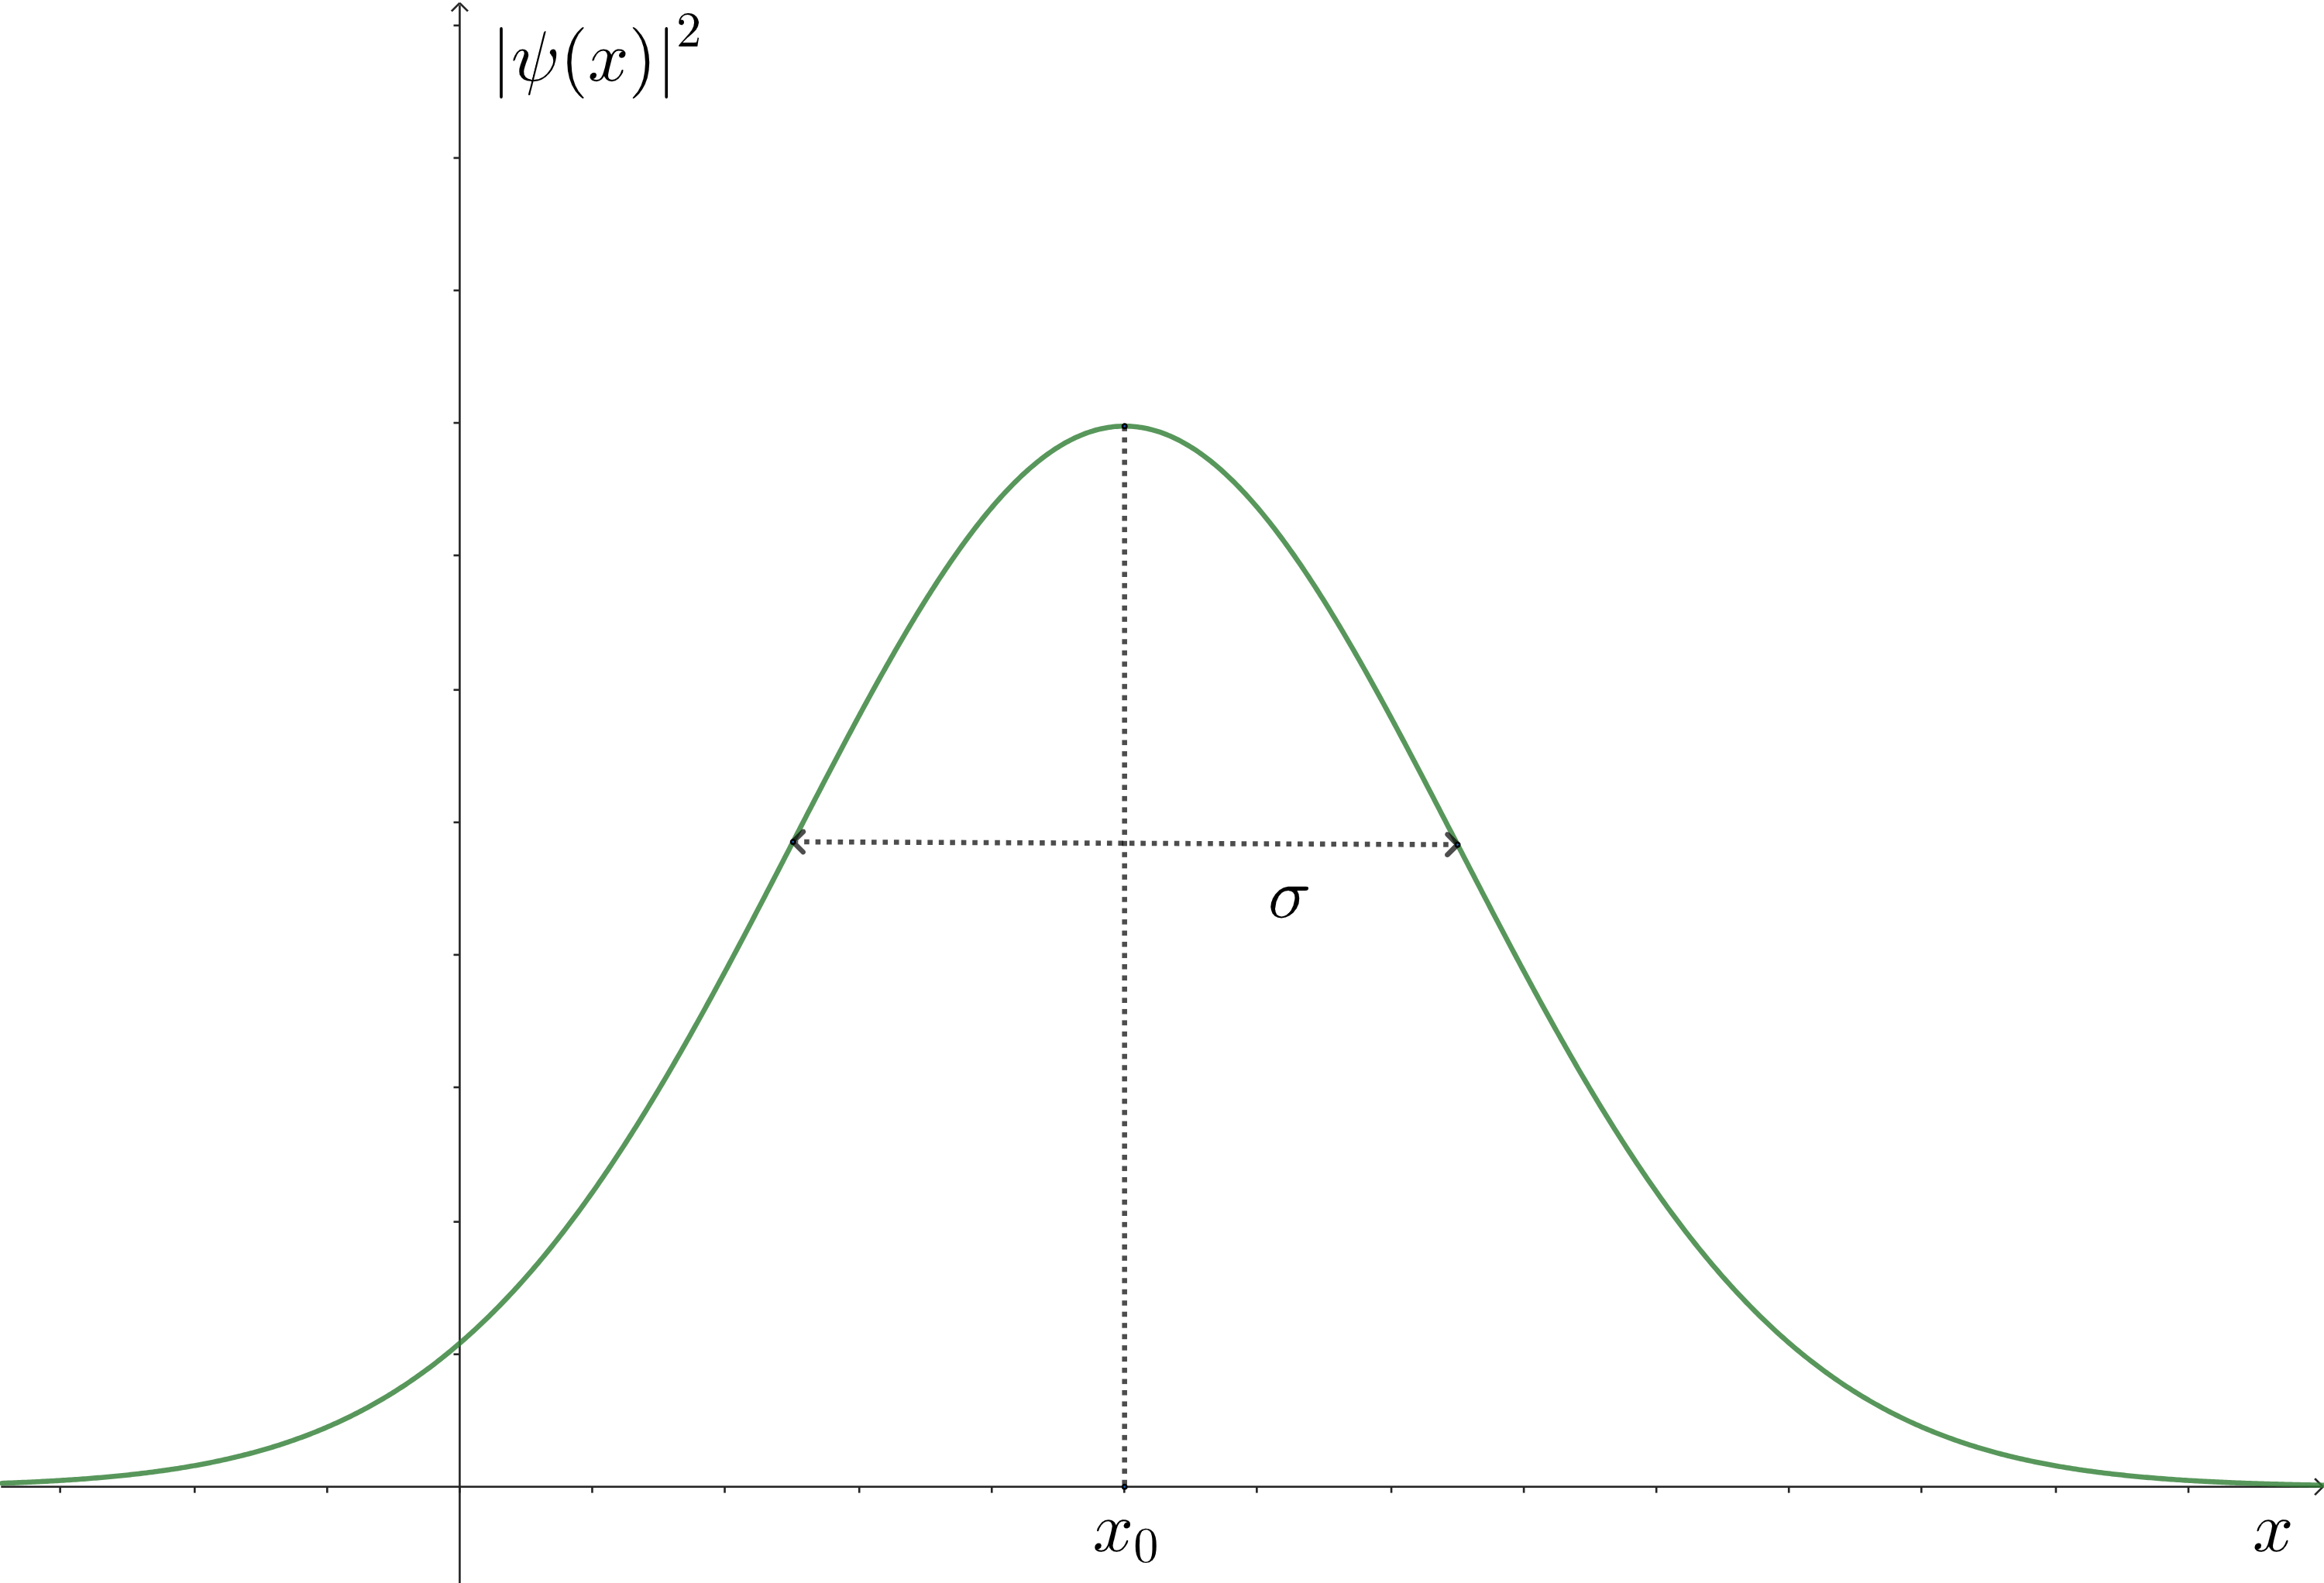
\includegraphics[scale = 3]{gaussian-wavepacket.png}
\end{center}
\par
Back to the use of Dirac notation, if we are give $\ketpsi \in \hilbert$, then
$$\brapsi = (\ketpsi)^{\dagger}$$
From the qubit system,
$$\ketpsi = \begin{pmatrix}
    \alpha \\ \beta
\end{pmatrix} \to \brapsi = \begin{pmatrix}
    \conj{\alpha} & \conj{\beta}
\end{pmatrix} = \conj{\alpha}\bra{0} + \conj{\beta}\bra{1}$$
From the 1D continuous system,
$$\ketpsi = \intR \psi(x)\ketx \dx \to \brapsi = \intR \conj{\psi}(x)\brax \dx$$
Then, given another quantum state in the discrete case:
$$\ketphi = \begin{pmatrix}
    \gamma \\ \zeta
\end{pmatrix}$$
We have
$$(\psi, \phi) = \conj{\alpha}\gamma + \conj{\beta}\zeta = \begin{pmatrix}
    \conj{\alpha} & \conj{\beta}
\end{pmatrix} \cdot \begin{pmatrix}
    \gamma \\ \zeta
\end{pmatrix} = \brapsi \cdot \ketphi = \braket{\psi}{\phi} = (\ketpsi, \ketphi)$$
In the continuous case, we have
$$(\psi, \phi) = \intR \conj{\psi}(x)\phi(x) \dx$$
Since the bra-ket notations are simply vectors, we also have the outer products between states, for example:
$$\dyad{0}{0} = \begin{pmatrix}
    1 \\ 0
\end{pmatrix} \begin{pmatrix}
    1 & 0
\end{pmatrix} = \begin{pmatrix}
    1 & 0 \\
    0 & 0
\end{pmatrix}$$
$$\dyad{\phi}{\psi} = \begin{pmatrix}
    \gamma \\ \zeta
\end{pmatrix}\begin{pmatrix}
    \conj{\alpha} & \conj{\beta}
\end{pmatrix} = \begin{pmatrix}
    \gamma\conj{\alpha} & \gamma\conj{\beta} \\
    \zeta\conj{\alpha} & \zeta\conj{\beta}
\end{pmatrix} \in \C^{2 \times 2}$$
% ----------------------------------------------------------------
\subsection{Postulate 3 - “公理”三}
After postulating the quantum system as a complex Hilbert space, with a quantum state being a normalized vector in this Hilbert space, we now wish to proceed to how to conduct a measurement on such a system, as we require measurement to obtain information. \par
In this case, we prepare a quantum system in state $\ketpsi \in \hilbert$, and let $\{\ket{x}\}_x$ to be an \impt{orthonormal basis} of $\hilbert$. From this setup, we know:
$$\braket{x}{x'} = \delta_{xx'} = \delta(x-x')$$
\begin{postulate}
    \raggedright
    A quantum system $\hilbert$ can be measured with respect to an orthonormal basis $\{\ket{x}\}_x$, such that the possible outcomes are labels $\{x\}_x$ with probability distribution/density
    $$ \Prob{x}_\psi = \abs{\braket{x}{\psi}}^2 $$
    This is also referred to as \uimpt{Born's Rule}. \\
    The post-measurement state upon receiving outcome $x$ is $\ket{x}$, this is equivalent to saying ``measurement changes the state'', or ``\uimpt{measurement corresponds to the collapse of the wavefunction}''
\end{postulate}
Note that a single quantum system can only produce a single outcome. If we wish to learn more about a state $\ketpsi$, we need multiple preparations and measurements to estimate $\Prob{x}_\psi$. \par
Now we wish to know, given an orthonormal basis $\{\ket{x}\}_x$ of the quantum system $\hilbert$, to which state will the wavefunction collapse?
\begin{definition}
    Quantum measurements with respect to an orthonormal basis are also called \uimpt{projective measurements}. Assume the orthonormal basis with resepct to which we are measuring is $\{\ket{x}\}_x$, we define a \uimpt{projector onto $\ket{x}$} to be:
    $$\proj{x} = \dyad{x}{x}$$
\end{definition}
We derive from Born's Rule:
\begin{align*}
    \Prob{x}_\psi &= \abs{\braket{x}{\psi}}^2 \\
    &= \braket{x}{\psi}^{*}\braket{x}{\psi} \\
    &= \braket{\psi}{x}\braket{x}{\psi} \\
    &= \mel{\psi}{\proj{x}}{\psi}
\end{align*}
If we wish to measure in another basis, we must represent the state in terms of the new basis first. This once again highlights that \impt{wavefunctions are dependent on the basis}. \par
In order for $\Prob{x}_\psi$ to be a probability distribution, two conditions must hold:
\begin{quote}
    1. $\Prob{x}_\psi \ge 0$ \\
    2. $\displaystyle \Sumi{x} \Prob{x}_\psi = 1$
\end{quote}
It is trivial that $\Prob{x}_\psi \ge 0$, as it is a complex number's norm's square. However, to satisfy the second condition, we require \impt{normalization}:
$$\Sumi{x} \Prob{x}_\psi = \Sumi{x} \abs{\braket{x}{\psi}}^2 = \Sumi{x} \abs{\psi(x)}^2 = 1$$
This derivation is natural from the fact that:
$$\ketpsi = \Sumi{x} \psi(x)\ket{x}$$
To deal with a continous Hilbert space, we may replace the summation symbol with the integral. \par
To a measurement, only the outcome and the probability of the outcome matter, therefore, \impt{global phases are physically irrelevant}. To show this, consider two quantum states where they only differ by a global phase $e^{\imag \varphi}$, that is, given:
$$\ketpsi \ne e^{\imag \varphi}\ketphi = \ketphi, \varphi \in \R, \text{ not a multiple of } 2\pi$$
If we wish to know the probability of outcome $x$ for the state $\ketphi$, we have:
\begin{align*}
    \Prob{x}_\phi &= \abs{\braket{x}{\phi}}^2 \\
    &= \abs{\mel{x}{e^{\imag \varphi}}{\psi}} \\
    &= \abs{e^{\imag \varphi}}^2 \abs{\braket{x}{\psi}}^2 \\
    &= \Prob{x}_\psi
\end{align*}
This derivation is natural because $e^{\imag \varphi}$ is a complex number with norm being $1$. \par
We may also describe the process of measurements in another way.
\begin{definition}
    An \uimpt{observable} $\mathcal{O}$ is a \uimpt{Hermitian operator}, where measuring $\mathcal{O}$ amounts to doing a \uimpt{projective measurement} with respect to the \uimpt{orthonormal basis of eigenvectors} of $\mathcal{O}$, and relabelling the outcome $x$ as $\lambda_x$
\end{definition}
Take a qubit as an example, a Pauli-Z measurement would amount to doing a projective measurement with respect to $\ket{0}$ and $\ket{1}$ as
$$Z = \begin{pmatrix}
    1 & 0 \\
    0 & -1
\end{pmatrix} = (+1)\begin{pmatrix}
    1 & 0 \\
    0 & 0
\end{pmatrix} + (-1) \begin{pmatrix}
    0 & 0 \\
    0 & 1
\end{pmatrix}$$
where $+1$ is the eigenvalue of eigenvector $\ket{0}$ and $-1$ is the eigenvalue of eigenvector $\ket{1}$. \\
Similarly, a Pauli-X measurement would amount to doing a projective measurement with respect to $\ketplus$ and $\ketminus$, with their respective eigenvalues to be $+1$ and $-1$. \\
In a continuous case, consider the position measurement as an example, where $\{\ket{x}\}_{x \in \R}$ is the position basis. We label $\lambda_x = x$, then the position observable is:
$$\oppos = \intR \lambda_x \dyad{x}{x} \dd x$$
\begin{definition}
    Given an observable $\mathcal{O}$ and a state $\ketpsi$, then the \uimpt{expected value} of this observable with respect to this state is:
    $$\expval{\mathcal{O}}_\psi = \ev{\mathcal{O}}{\psi}$$
\end{definition}
\begin{definition}
    The \uimpt{variance} of the above observable and the above state is:
    $$(\Delta \mathcal{O})_\psi^2 = \expval{\mathcal{O}^2}_\psi - (\expval{\mathcal{O}}_\psi)^2$$
\end{definition}
Once again, consider a general position state $\ketpsi = \intR \psi(x) \ket{x} \dd x$, and the above position observable. Then, the expected value of the position observable with respect to state $\ketpsi$ is:
\begin{align*}
    \expval{\oppos}_\psi &= \ev{\oppos}{\psi} \\
    &= \brapsi \intR x \dyad{x}{x} \dd x \ketpsi \\
    &= \intR x \dyad{\psi}{x}\dyad{x}{\psi} \dd x \\
    &= \intR x \conj{\psi}(x) \psi(x) \dd x \\
    &= \intR x \abs{\psi(x)}^2 \dd x
\end{align*}
We often wish to properly represent the outcome or the \impt{post-measurement} state. In this case, if we denote the initial state to be $\ketpsi$, and the post-measurement state to be $\ket{\psi'}$, then we have
$$\ket{\psi'} = \frac{\proj{i}\ketpsi}{\sqrt{\Prob{\lambda_i}}}$$
An additional useful operator is the \impt{reflection (parity)} operator, where we denote it as $\hat{R}$:
$$\hat{R} = \intR \dyad{x}{-x} \dd x$$
and has the following properties:
\begin{quote}
    1. $\hat{R}\ket{x} = \ket{-x}$. \\
    2. $\hat{R}^2 = \mathbb{I}$. \\
    3. $\hat{R}\oppos\hat{R} = -\oppos$
\end{quote}

\subsection{Postulate 4 - “公理”四}
So far, we have postulated the settings of a physical system in a quantum-mechanic way. We have defined a \impt{quantum system} in terms of a Hilbert space, a \impt{quantum state} in terms of a normalized vector in such a Hilbert space, and how the system can be \impt{measured} with respect to an orthonormal basis which relates to an \impt{observable} represented as a Hermitian operator. \par
Furthermore, we also hope describe how such a system evolves in time. This is, we wish to understand the \impt{dynamics} of a quantum system.
\begin{postulate}
    Closed quantum systems that do not have interactions with other quantum systems, evolve \uimpt{reversibly} and the \uimpt{reversible evolution} of a state $\ketpsi \in \hilbert$ is expressed as a \uimpt{unitary transformation}.
    $$\ketpsi \to \opuni \ketpsi, \opuni \in \opuni(\hilbert)$$
\end{postulate}
Here, since \hyperref[subsec:unitary]{\textcolor{cyan}{unitary matrices}} are invertible, we have $\opuni^{-1} = \conjt{\opuni}$ which implies a reversible evolution. \par
An example of such unitary operators is the Hadamard operator, the evolution under the Hadamard gate is as follows:
\begin{align*}
    H \ket{0} &= \frac{1}{\sqrt{2}} \begin{pmatrix}
        1 & 1 \\
        1 & -1
    \end{pmatrix} \begin{pmatrix}
        1 \\ 0
    \end{pmatrix} = \frac{1}{\sqrt{2}} \begin{pmatrix}
        1 \\ 1
    \end{pmatrix} = \ketplus \\
    H \ket{1} &= \ketminus \\
    H \ketplus &= \ket{0} \\
    H \ketminus &= \ket{1}
\end{align*}
It is easily seen that the Hadamard preserves the inner product as $\braket{0}{1} = \braket{+}{-} = 0$
\subsubsection{Schr\"odinger's Equation - 薛定谔方程}
Let $\ket{\psi(t)}$ be a \impt{time-dependent} state evolving \impt{unitarily} in a closed system. At time $t_0$, we denote the state as $\ket{\psi(t_0)}$ and after time continues to $t$, we have observed the evolution as such $\ket{\psi(t_0)} \mapsto \ket{\psi(t)}$. \par
We wish to understand what equation of motion governs the evolution. The evolution defines the equation of motion, while the equation of motion implies evolution. An \impt{equation of motion} is a differential equation in time defining the evolution. \par
\begin{definition}
    Let $\opuni(t, t_0)$ be an unitary operator that time-evolves an initial state at $t_0$: $\ket{\psi(t_0)}$ to the evolved state at $t$: $\ket{\psi(t)}$. We call such an operator the \uimpt{propagator}.
    $$\opuni(t, t_0)\ket{\psi(t_0)} = \ket{\psi(t)}$$
\end{definition}
With this setup, we now derive the Schr\"odinger's equation. \par
We take the time-derivative $\dd t$ of the state $\ket{\psi(t)}$:
\begin{align*}
    \pdv{t} \ket{\psi(t)} &= \lim_{\Delta \to 0} \frac{\ket{\psi(t + \Delta)} - \ket{\psi(t)}}{\Delta} \\
    &= \lim_{\Delta \to 0} \frac{\opuni(t+\Delta, t)\ket{\psi(t)} - \ket{\psi(t)}}{\Delta} \\
    &= (\lim_{\Delta \to 0} \frac{\opuni(t+\Delta, t) - \id}{\Delta})\ket{\psi(t)}
\end{align*}
For easier interpretation, we temporarily denote $\displaystyle G = \lim_{\Delta \to 0} \frac{\opuni(t+\Delta, t) - \id}{\Delta}$, which is a linear operator. So, we have $\pdv{t} \ket{\psi(t)} = G \ket{\psi(t)}$. \par
We first observe that $G$ is \impt{anti-Hermitian}, proven through the following:
\begin{align*}
    \pdv{t} \braket{\psi(t)} &= 0 \\
    (\pdv{t}\bra{\psi(t)})\ket{\psi(t)} + \bra{\psi(t)}(\pdv{t} \ket{\psi(t)}) &= 0 \\
    \ev{\conjt{G}}{\psi(t)} + \ev{G}{\psi(t)} &= 0 \\
    \conjt{G} + G &= 0
\end{align*}
We now have the equation of motion: $\pdv{t} \ket{\psi(t)} = G\ket{\psi(t)}$, where $G$ is anti-Hermitian. \par
By convention, we multiply the equation of motion by $\imag \hbar$. This would have the effect of $G \mapsto \imag G$ which is now Hermitian. In this case, we define the \impt{Hamiltonian} as 
$$\hat{H} := \imag \hbar G$$
Then, we finally obtain the \impt{time-dependent Schr\"odinger's equation}:
$$\hat{H}\ket{\psi(t)} = \imag \hbar \pdv{t} \ket{\psi(t)}$$
This is the \impt{equation of motion of quantum states in a closed system}. \par
Since $\hat{H}$ is Hermitian, it can be interpreted as an observable, the physical quantity measured when measuring observable $\hat{H}$ is the \impt{total energy of the quantum system}. In general, the Hamiltonian can be time-dependent, but mostly time-independent (which is, $\hat{H}(t) \equiv \hat{H}$). In order to know what Hamiltonian maps to what evolution/propagator $\opuni(t, t_0)$, we need to solve the Schr\"odinger's equation for different Hamiltonians.

\subsection{Postulate 5 - “公理”五}
\begin{postulate}
    Let $A$ and $B$ be quantum systems associated with $\hilbert: \hilbert_A, \hilbert_B$. The \uimpt{composite system} $AB$ is associated with the Hilbert space:
    $$\hilbert_{AB} = \hilbert_A \otimes \hilbert_B$$
\end{postulate}
Take 2 qubits as an example, where the composite quantum system is essentially $\C^2 \otimes \C^2$. Then, the notation of a state in this system can be:
$$\ket{0}_A \otimes \ket{0}_B = \ket{0} \otimes \ket{0} = \ket{0}_A\ket{0}_B = \ket{0}\ket{0} = \ket{00}_{AB} = \ket{00}$$
For the same composite quantum system, consider the following state:
$$\ket{\psi^{00}}_{AB} = \frac{1}{\sqrt{2}}(\ket{00} + \ket{11})$$
It is not possible to write the quantum state in the form of $\ketpsi_A \otimes \ketphi_B$ even though it is a valid state of the composite system.
\begin{definition}
    For all possible/valid states in a composite quantum system, we define the states that can be written as the tensor product of quantum states of component systems (e.g. $\ketpsi_A \otimes \ketphi_B$) as \uimpt{product states}, and those that cannot be written in such a form as \uimpt{entangled states}.
\end{definition}
If we have an orthonormal basis $\{\ket{k}_A\}_k$ on $\hilbert_A$ and $\{\ket{j}_B\}_j$ on $\hilbert_B$, then $\{\ket{k}_A\ket{j}_B\}_{(k, j)}$ is an orthonormal basis of $\hilbert_A \otimes \hilbert_B$. A general state of such a system can be represented as:
$$\ketpsi_{AB} = \Sumi{k, j}\psi(k, j)(\ket{k}_A \otimes \ket{j}_B)$$
$$\ketpsi_{AB} = \intR\intR \psi(x, y)(\ket{x} \otimes \ket{y}) \dd x \dd y$$
If $\dim \hilbert_A, \dim \hilbert_B < \infty$, then $\dim (\hilbert_A \otimes \hilbert_B) = \dim \hilbert_A \cdot \dim \hilbert_B$. \par
Consider a local linear operator $M_A$ on subsystem $\hilbert_A$, then the corresponding global operator on the composite system is:
$$M_{AB} = \Sumi{m} \alpha_m S_A^{(m)} \otimes T_B^{(m)}$$
Then for a generic state, we have
$$M_{AB}\ketpsi_{AB} = \Sumi{m} \alpha_m \Sumi{k, j} \psi(k, j)(S_A^{(m)} \ket{k}_A) \otimes (T_B^{(m)} \ket{j}_B)$$
This indicates that if subsystem $A$ undergoes a unitary evolution $\opuni_A$ while $B$ does not undergo any evolution, the evolution on $AB$ is unitary $\opuni_{AB} = \opuni_A \otimes \id_B$. However, the converse is not true, that is, if the entire system undergoes a generic unitary evolution ($\opuni_{AB} \in \opuni(\hilbert_A \otimes \hilbert_B)$), it does not imply that each subsystem undergoes a unitary evolution. \par
Furthermore, if we consider a local projective measurement, that is say, let $\{\proj{A}^{(k)}\}_k$ be projectors of local measurements on $A$, then the operator on $AB$ is thus: $\{\proj{A}^{(k) \otimes \id_B}\}_k$. Almost the same rules apply to composite systems when compared to a single system:
\begin{quote}
    1. Born's Rule: $\Prob{k_A}_{\psi_{AB}} = \brapsi_{AB} \proj{A}^{(k)} \otimes \id_B \ketpsi_{AB}$. \\
    2. Post-measurement state upon receiving outcome $k_A$: $\frac{\proj{A}^{(k)} \otimes \id_B \ketpsi_{AB}}{\sqrt{\Prob{k_A}_{\psi_{AB}}}}$
\end{quote}
An example operator on composite systems is the controlled-NOT gate (a.k.a CNOT). It works on 2 qubits, and it is an operator of the following form:
$$\text{CNOT} = \dyad{0}{0} \otimes \id + \dyad{1}{1} \otimes X$$
The gate takes in 2 qubits, the first one being the ``control'' and the second being the ``target''. Its function is to flip the target if the control is $1$. Thus, in general, the operator does the following operations:
\begin{quote}
    1. $\ket{00} \mapsto \ket{00}$ \\
    2. $\ket{01} \mapsto \ket{01}$ \\
    3. $\ket{10} \mapsto \ket{11}$ \\
    4. $\ket{11} \mapsto \ket{10}$
\end{quote}
Explicitly, the CNOT gate should be a $4 \times 4$ matrix of the following form:
$$\text{CNOT} = \begin{pmatrix}
    1 & 0 & 0 & 0 \\
    0 & 1 & 0 & 0 \\
    0 & 0 & 0 & 1 \\
    0 & 0 & 1 & 0
\end{pmatrix}$$

\subsection{Bloch Sphere - 布洛赫球面}
To start with this concept, we first introduce the basic single-qubit gates: Pauli-X, Pauli-Y, and Pauli-Z. The matrix form, given in the computational Z basis, are:
$$X = \begin{pmatrix}
    0 & 1 \\
    1 & 0
\end{pmatrix}, Y = \begin{pmatrix}
    0 & -\imag \\
    \imag & 0
\end{pmatrix}, Z = \begin{pmatrix}
    1 & 0 \\
    0 & -1
\end{pmatrix}$$
Any pure state of a qubit can be described and visualized as a \impt{point on a 3D sphere of radius 1}. This is demonstrated as follows. \par
First, any pure state of a single qubit can be written as:
$$\ketpsi = \alpha \ket{0} + \beta \ket{1}$$
with $\abs{\alpha}^2 + \abs{\beta}^2 = 1$. Represent the coefficients (a complex number) in product form: $\alpha = \abs{\alpha}e^{\imag \omega_1}, \beta = \abs{\beta}e^{\imag \omega_2}$. So we have:
\begin{align*}
    \ketpsi &= \alpha \ket{0} + \beta \ket{1} \\
    &= |\alpha|e^{\imag \omega_1}\ket{0} + \abs{\beta}e^{\imag \omega_2}\ket{1} \\
    &= \abs{\alpha}\ket{0} + \abs{\beta}e^{\imag (\omega_2 - \omega_1)}\ket{1}
\end{align*}
where $e^{-\imag \omega_1}$ is a global phase (it does not change the state), and $\phi = \omega_2 - \omega_1$ (the relative phase between two basis states). \par
Since we want to represent this state on the surface of the sphere, we use spherical coordinates where $\theta \in [0, \pi]$ and $\phi \in [0, 2\pi)$. \par
Right now, we have $\ketpsi = \abs{\alpha}\ket{0} + \abs{\beta}e^{\imag\phi}\ket{1}$. We wish to justify that this state can be written as
$$\ketpsi = \cos(\frac{\theta}{2})\ket{0} + \sin(\frac{\theta}{2})e^{\imag \phi}\ket{1}$$
so that we can use $\theta$ and $\phi$ for spherical-coordinate representation. \par
So far, with $\ketpsi$ being a quantum state, it is trivial to see that we can easily denote $\abs{\alpha}$ as $\cos(x)$ and $\abs{\beta}$ as $\sin(x)$. Thus, we need to justify why $x$ here must be $\frac{\theta}{2}$ instead of some other value. We should start by considering what mathematical conditions $\abs{\alpha}$ and $\abs{\beta}$ should satisfy:
\begin{quote}
    1. $0 \le \abs{\alpha}, \abs{\beta} \le 1$. \\
    2. $\abs{\alpha}, \abs{\beta}$ should uniquely correspond to a $\theta$.
\end{quote}
This indicates that $\cos(x), \sin(x)$ must be within the range $0$ to $1$ while $x \in [0, \pi]$. This condition shows that if $x$ is a factor of $\theta$, the factor must be exactly $\frac{1}{2}$. Thus, we can properly justify why $\abs{\alpha} = \cos(\frac{\theta}{2})$ and $\abs{\beta} = \sin(\frac{\theta}{2})$. \par
Therefore, now when we consider the eigenstates (computational basis) of the Pauli-Z, -X, -Y operators on this Bloch sphere, we can see why the operators are named this way:
\begin{quote}
    1. Pauli-Z: has computational basis $\ket{0}$ and $\ket{1}$.
    $$\ket{0} = (\theta = 0, \phi); \ket{1} = (\theta = \pi, \phi)$$
    we see that $\ket{0}$ lies on the positive $z$-direction, and $\ket{1}$ lies on the negative $z$-direction; \\
    2. Pauli-X: has computational basis $\ketplus$ and $\ketminus$.
    $$\ketplus = (\theta = \frac{\pi}{2}, \phi = 0); \ketminus = (\theta = \frac{\pi}{2}, \phi = \pi)$$
    we see that $\ketplus$ lies on the positive $x$-direction, and $\ketminus$ lies on the negative $x$-direction; \\
    3. Pauli-Y: has computational basis $\ket{+\imag}$ and $\ket{-\imag}$.
    $$\ket{+\imag} = (\theta = \frac{\pi}{2}, \phi = \frac{\pi}{2}); \ket{-\imag} = (\theta = \frac{\pi}{2}, \phi = \frac{3\pi}{2})$$
    we see that $\ket{+\imag}$ lies on the positive $y$-direction, and $\ket{-\imag}$ lies on the negative $y$-direction.
\end{quote}
\begin{center}
    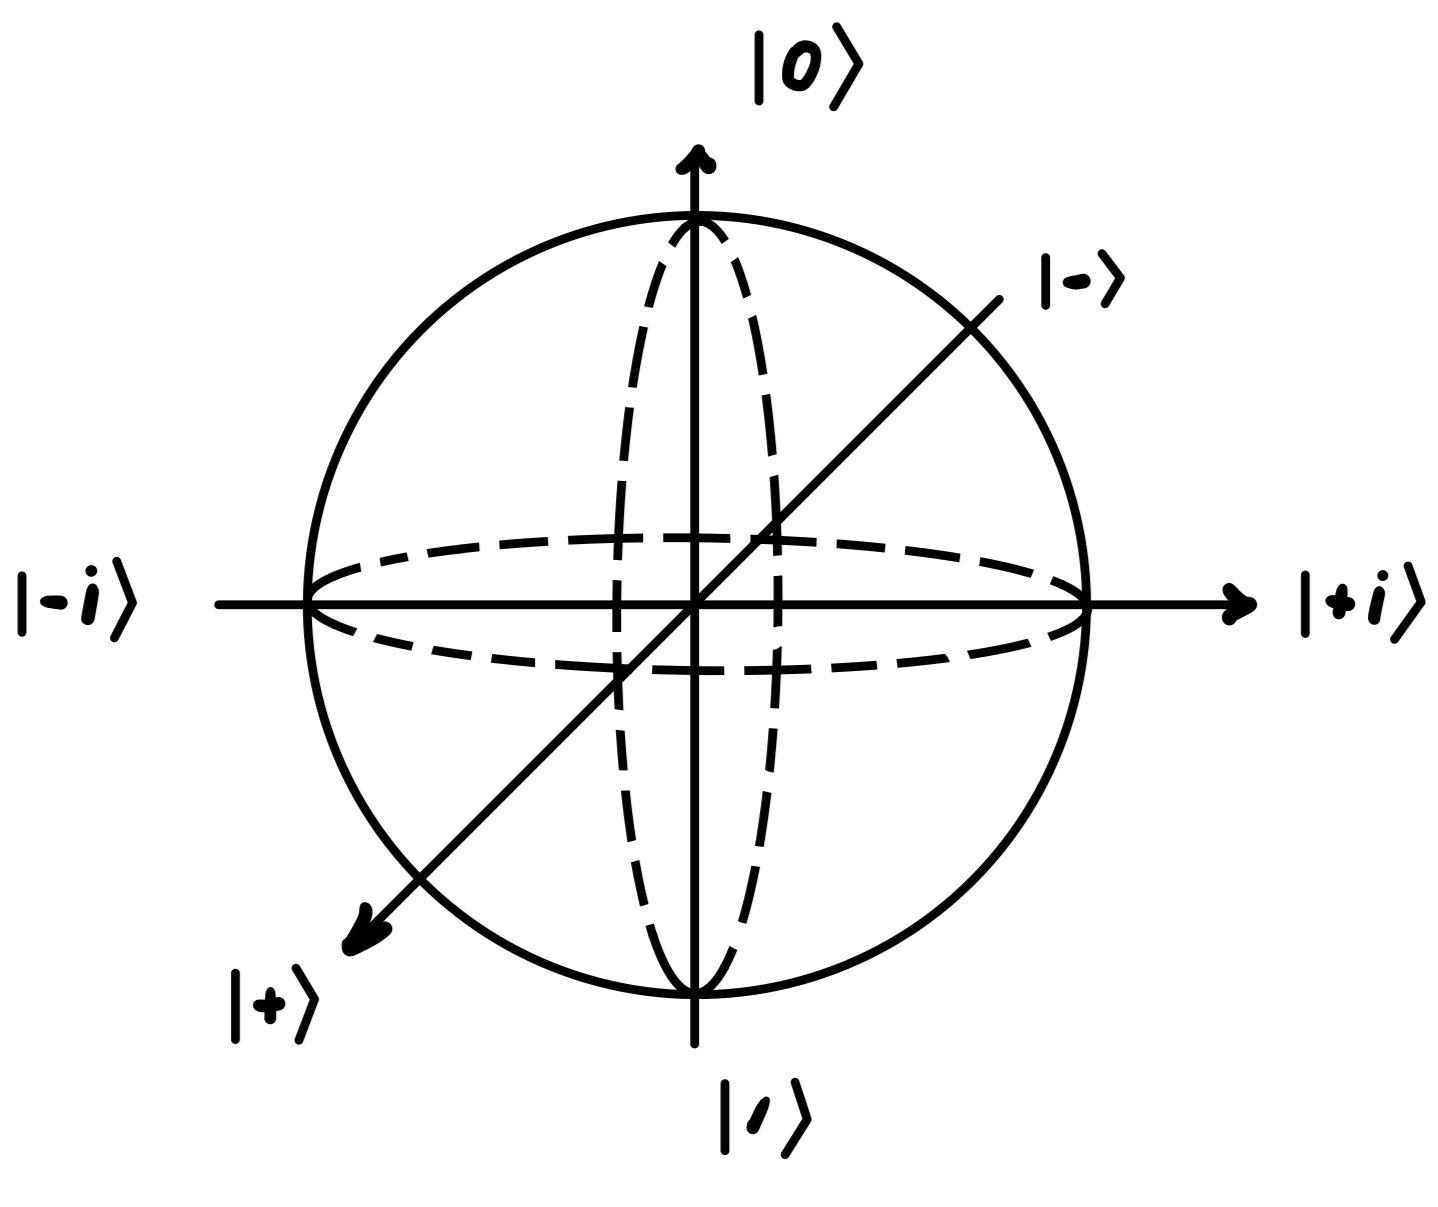
\includegraphics[scale = 0.25]{bloch-sphere.png}
\end{center}
It is helpful to know the following relationship:
\begin{align*}
    \ketpsi &= \alpha \ket{0} + \beta \ket{1} \\
    &= \frac{\alpha + \beta}{\sqrt{2}}\ketplus + \frac{\alpha - \beta}{\sqrt{2}}\ketminus
\end{align*}

\newpage